% Project - Technical Documentation
%
% Data Acquisition Technologies and Sensor Networks
% Jacobs University Bremen
% Supervisor: Prof. Dr. Fangning Hu
%
% Created on November 20, 2019
%
% Authors:
%   Ralph Florent <r.florent@jacobs-university.de>
%   Diogo Cosin <d.ayresdeoliveira@jacobs-university.de>
%   Eno Ciraku <e.ciraku@jacobs-university.de>

% ==============================================================================
% START: Methodology
% ==============================================================================

\section{Methodology}
In this section, we describe the techniques and strategies as well as the procedural methods used to implement the core functionality of this project. This description includes the components of the system, the workflow diagram, the third-party libraries, the algorithm and data structure, and finally, the code implementation.

It is important to stand out the fact that we use external resources to come up with daily results in terms of programming tools and full-on working devices. That is, before adventuring into using the materials and devices as well as certain software tools, different research sources were consulted. Some of these resources are: the datasheets of the prebuilt modules of the materials, the assistance of the instructor and teaching assistants (TAs), search engines (mainly Google Search/Internet), and finally some related books and references (e.g. materials provided by the professor).

Being exceptionally helpful, these resources have been the source of truth for any decision-making regarding the correct use of the hardware modules.

\subsection{Components of the prototype}
Roughly speaking, Smart Outlet comprises 3 (three) principal modules:
\begin{itemize}
    \item \textbf{\textit{Webduino}}: a low-level, modular circuitry formed by an Arduino and a network of sensors. The Arduino board, a microcontroller, acts as a supervisor of micro tasks. Being the core component of the hardware systems, it controls the different input/ouput functions of the connected chips.
    \item \textbf{\textit{Web API}}: an API service attending HTTP requests from the \emph{webduino} (its only consumer). It coordinates the communication between the Wi-Fi module of the webduino (client) over the air medium (wireless) and the available API resources on an HTTP server. The API service contains various layers of interactons, including the database for data persistence.
    \item \textbf{\textit{Web APP}}: (short for web application) a single page application (SPA) to visualize the historical content or performed actions during the webduino's operations. It allows user-friendly interactions between an end-user and the prototype itself. The web app is also responsive. That is, it can be accessed and used via mobile devices (tablets, smartphones, etc.).
\end{itemize}

Each one of these modules deep down contains a set of characteristics that requires more than a brief description to highlight their corresponding functionality. However, in this document, we intend to only explain how to connect them together and make them work properly as a whole. We indeed provide full access to the online repository as specified in Appendix \ref{sec:code-repo} so that anyone can dig any further into the datasheets if needs be.

\subsection{Workflow diagram}
The Smart Outlet project has an easy-to-understand workflow. This workflow explains how each module is connected to each other (not fully as in a mesh connection) and performs a specific task. In the section, we provide a diagram and explain the corresponding role of the inner contents taking part in that workflow in other to achieve the complete functionality of Smart Outlet as a whole.

As shown in Figure \ref{fig:workflow-diagram}, the workflow diagram consists of the following parts:
\begin{itemize}
    \item some end-user devices accessing the web application
    \item a server infrastructure attending requests over TCIP/IP network
    \item the webduino connected to the same network waiting to update the states of the outlets, if any.
\end{itemize}

\noindent
How do the components interact with each other?
\begin{enumerate}
    \item given the initial conditions, where all the components are up and running properly\footnote{The devices (database, API web service, webduino) should be powered on and running. Each device should be assigned a local IP address and should be reachable by other devices over the network.}
    \item the webduino will constantly attempt to request the last states of the power outlets from the web API service. Once obtained the data over Wi-Fi, it proceeds by updating the states of the relays, which in turn will open or close the switch of a power outlet.
    \item A user accessing web browser may view the last updates of the power outlets. When a user updates\footnote{Set an update for a power outlet is basically to change its state from ON-OFF or viceversa.} the state of an outlet, the changes are saved into the database through the API service and immediately (~2 seconds) reflected in the webduino.
    \item The historical records can also be visualized on a separate views using both a tabular form and a scatter plot.
\end{enumerate}

\begin{figure}[!ht]
    \centering
    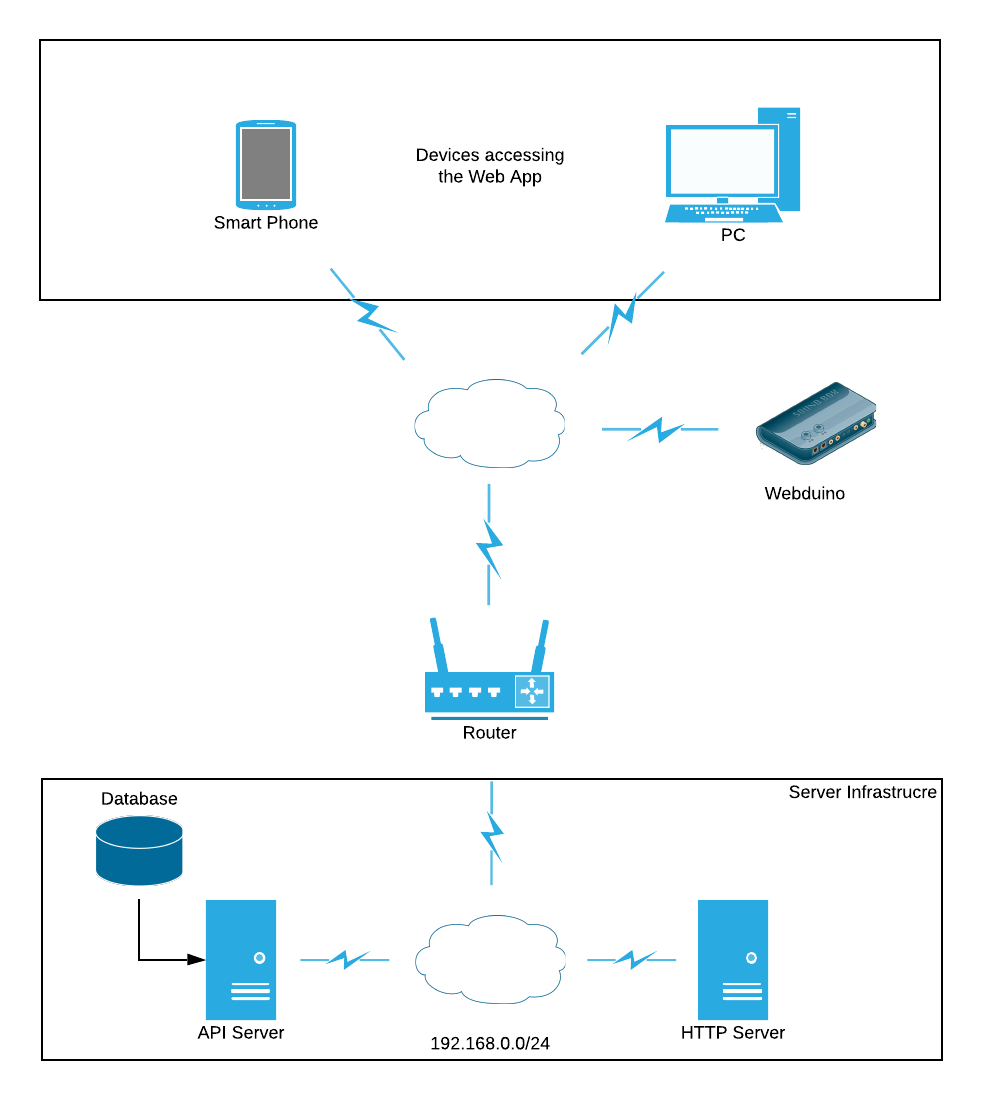
\includegraphics[scale=0.33]{workflow.png}
    \caption{Workflow diagram \\ (credits: made with \emph{Lucidchart})}
    \label{fig:workflow-diagram}
\end{figure}

\subsection{Algorithm and data structure}

\subsection{Code implementation}
% ==============================================================================
% END: Methodology
% ==============================================================================